\section{Polynomial Rings} 

  In ring theory, the idea of \textit{adjoining} an existing ring $R$ with an arbitrary element $x$ will appear frequently. That is, given a ring $R$ and some $x$, can we try and construct a new ring $S$, denoted $R[x]$ that is the minimal ring containing both $R$ and $x$? What kind of elements would be in $R[x]$? 
  \begin{enumerate}
    \item Since $R \subset R[x]$, it must be the case that for $a \in R$, $a \in R[x]$. 
    \item Since $x \in R[x]$, it must be the case that $a x \in R[x]$ for all $a \in R$. 
    \item $x \times x = x^2 \in R[x]$, so it must be the case that $a x^2 \in R[x]$ 
    \item In general, for any $n \in \mathbb{N}$, $x^n \in R[x]$, so it must be the case that $a x^n \in R[x]$. 
  \end{enumerate}
  If we add these terms up, we have elements of the general form 
  \begin{equation}
    a_n x^n + a_{n-1} x^{n-1} + \ldots + a_1 x + a_0 
  \end{equation}
  This is what we refer to as a polynomial, and it indeed does have a ring structure. More generally, given a set of elements $S = \{x_1, \ldots, x_n\}$, $R[S]$ can be defined accordingly. Now let's formally define them. 

  \begin{definition}[Polynomial Ring]
    Given ring $R$ and a set of \textbf{indeterminates} $S = \{x_1, \ldots, x_n\}$, the \textbf{ring of polynomials} $R[S] = R[x_1, \ldots, x_n]$ is defined in the equivalent ways. 
    \begin{enumerate}
      \item It is the minimal ring containing $R$ as a subring and $S$. 
      \item It is the ring of formal expressions of the form 
      \begin{equation}
        f(x_1, \ldots, x_n) = \sum_{0 \leq k_i \leq n} a_{k_1 \ldots k_n} x_1^{k_1} x_2^{k_2} \ldots x_n^{k_n}, \quad a_i \in R
      \end{equation}
      which for univariate polynomials simplifies to 
      \begin{equation}
        f(x) = a_nx^n + a_{n-1}x^{n-1} + \dots + a_1 x + a_0, \quad a_i \in R
      \end{equation}
    \end{enumerate}
    From both definitions is becomes clear through the ring properties that 
    \begin{enumerate}
      \item Addition is defined component-wise: $a x^i + b x^i = (a + b) x^i$. 
      \item Multiplication is defined component-wise: $x^i x^j = x^{i + j}$. 
      \item Additive and multiplicative identities is $0$ and $1$. 
    \end{enumerate}
  \end{definition}

  Note that $x$ is just a formal symbol, whose powers $x^i$ are just placeholders for the corresponding coefficients $a_i$ so that the given formal expression is a way to encode the finitary sequence. $(a_0, a_1, a_2, ..., a_n)$. Two polynomials are equal if and only if the sequences of their corresponding coefficients are equal. Also note that unlike a function, which we write as $f$, for a polynomial we should write the indeterminate $f(x)$. We can however interpret $f(x)$ as a function as well (which may not be unique), and doing so allows us to determine special properties of $f(x) \in R[x]$. Before we move on, let's get some terms out of the way. 

  \begin{definition}[Some Terms for Polynomials]
    Given a univariate polynomial $f(x) \in R[x]$. 
    \begin{enumerate} 
      \item The \textbf{leading coefficient} is the last nonzero coefficient  
      \item The \textbf{degree} of $f$---denoted $\deg f$---is the index of the leading coefficient.
      \item A \textbf{monomial} is a polynomial of a single term $a_j x^j$. 
      \item A \textbf{linear} polynomial is a polynomial of degree 1. 
      \item A \textbf{quadratic} polynomial is a polynomial of degree 2. 
      \item A \textbf{cubic} polynomial is a polynomial of degree 3. 
    \end{enumerate}
  \end{definition}

  We need to be very careful about the properties that hold for polynomials, as they may not be intuitive. For example, for certain finite fields (which are rings), some formally different polynomials may be indistinguishable in terms of mappings.\footnote{$x$ and $x^2$ are equivalent in  $\mathbb{Z}_2 [x]$. } Second, a polynomial may have more roots than its degree. Therefore, we will work in different rings $R$ and provide conditions where our intuition is true in $R[x]$. It is clear that if you have two polynomials of degree $n$ and $m$, their sum may be degree $k < n, m$. This is not always true for multiplication. There is a simple condition in which the degree is additive, however. 

  \begin{lemma}[Bounds on Degrees From Operations]
    Given that $R$ is a ring and $f, g \in R[x]$, 
    \begin{equation}
      \deg(f+g) \leq \max\{\deg f, \deg g\}
      \deg(fg) \leq \deg f \deg g
    \end{equation}
  \end{lemma}
  \begin{proof}
    Trivial. 
  \end{proof}

  Unsurprisingly, the properties of the base ring $R$ determines the properties on $R[x]$, and we will explore more of this later. Finally, let's view polynomials as functions $f: R \to R$, which will allow us to talk about their \textit{roots}. 

  \begin{definition}[Polynomial Root]
    An element $r \in R$ is a \textbf{root} of polynomial $f \in R[x]$ if and only if 
    \begin{equation}
      f(r) = 0
    \end{equation}
  \end{definition}

  \begin{figure}[H]
    \centering 
    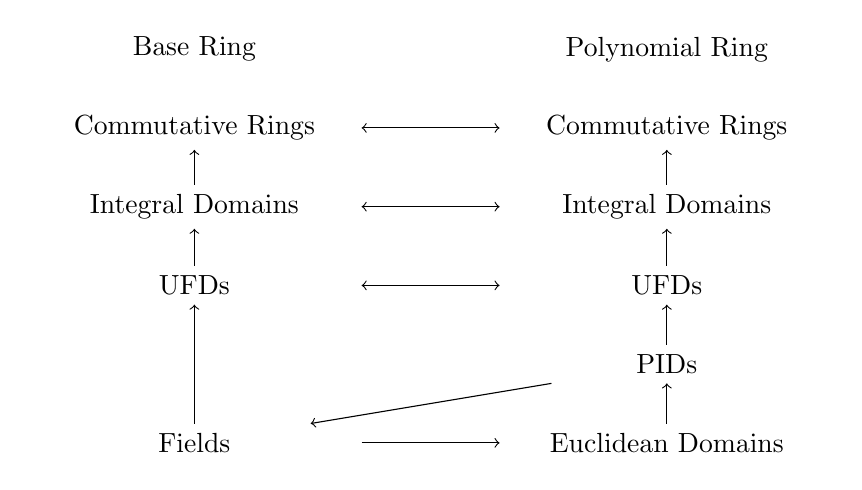
\begin{tikzpicture}[
      node distance=2cm,
      box/.style={
          text width=4cm,
          align=center
      }
      ]
      % Nodes for ring types
      \node[box] (base) at (-3,0) {Base Ring};
      \node[box] (poly) at (3,0) {Polynomial Ring};

      \node[box] (comm) at (-3,-1) {Commutative Rings};
      \node[box] (p_comm) at (3,-1) {Commutative Rings};
      \node[box] (int) at (-3,-2) {Integral Domains};
      \node[box] (p_int) at (3,-2) {Integral Domains};
      \node[box] (ufd) at (-3,-3) {UFDs}; % Added UFD between ID and PID
      \node[box] (p_ufd) at (3,-3) {UFDs}; % Added UFD between ID and PID
      \node[box] (field) at (-3,-5) {Fields}; % Moved Fields down
      \node[box] (p_pid) at (3,-4) {PIDs}; % Moved PID down
      \node[box] (p_euc) at (3,-5) {Euclidean Domains}; % Moved ED down
      
      % Left path arrows
      \draw[<-] (comm) -- (int);
      \draw[<-] (int) -- (ufd);
      \draw[<-] (ufd) -- (field);

      \draw[<-] (p_comm) -- (p_int);
      \draw[<-] (p_int) -- (p_ufd);
      \draw[<-] (p_ufd) -- (p_pid);
      \draw[<-] (p_pid) -- (p_euc);

      \draw[<->] (comm) -- (p_comm);
      \draw[<->] (int) -- (p_int);
      \draw[<->] (ufd) -- (p_ufd);
      \draw[->] (p_pid) -- (field);
      \draw[->] (field) -- (p_euc);
    \end{tikzpicture}
    \caption{Basic hierarchy of rings with UFDs included.} 
    \label{fig:poly_hierarchy}
  \end{figure}

\subsection{Commutative Polynomial Rings}

  We begin our study by looking at commutative polynomial rings. The first order of business is to be able to tell when such $R[x]$ is commutative. There is a simple condition for this. 

  \begin{theorem}[Conditions for $R\lbrack x \rbrack$ to be Commutative]
    Let $R$ be a ring and $S = \{x_1, \ldots, x_m\}$ be a finite set of indeterminates. $R$ is a commutative ring iff $R[x]$ is a commutative ring. 
  \end{theorem}
  \begin{proof}
    We prove bidirectionally. 
    \begin{enumerate}
      \item $(\rightarrow)$ If $R$ is commutative then given $a, b \in R$, we have $(ax^i) (b x^j) = a (x^i b) x^j = (ab)(x^i x^j) = (ba) (x^j x^i) = (b x^j) (a x^i)$, and so from distributive property $R[x]$ is commutative. 
      \item $(\leftarrow)$ This is trivial since given $R[x]$ commutative, take $a, b \in R \subset R[x]$, and so $ab = ba$ in $R[x]$ implies commutativity in $R$. 
    \end{enumerate}
  \end{proof}

  Now we associate long division with Euclidean domains, and this is the case in the integers. However, for polynomials, we can state a slightly weaker form in that we can divide any polynomial by not just any other polynomial, but a \textit{monic} polynomial. 

  \begin{theorem}[Division Algorithm Exists for Monic Divisors]
    \label{thm:poly-long-division}
    Given any ring $R$, with $f(x), d(x) \in R[x]$ where the leading coefficient of $d(x)$ is a unit, a division algorithm exists. That is, we can find a $q(x), r(x) \in R$ where 
    \begin{equation}
      f(x) = q(x) d(x) + r(x), \qquad 0 \leq \deg{r(x)} < \deg{d(x)}
    \end{equation}
  \end{theorem}
  \begin{proof}
    We construct how to do so. This is because at each step, you only need to divide the leading coefficient of the divisor into the leading coefficient of the polynomial you have left. 
  \end{proof}

  \begin{example}[Polynomial Long Division] 
    We apply the steps in the proof above to the example. 
    \begin{center}
      \polylongdiv{x^3 + 4x^2 - x + 7}{x - 2}
    \end{center}
  \end{example} 

  Now let's introduce polynomial roots and how they relate to the factors and evaluation of a function $f(x)$. 

  \begin{corollary}[Root-Factor Theorem]
    Given a commutative ring $R$ and $f(x) \in R[x]$, $(x - c)$ is a factor of $f(x)$, i.e. can be factored into 
    \begin{equation}
      f(x) = (x - c) q(x) 
    \end{equation}
    for some $q(x) \in R[x]$ of degree $\deg(f) - 1$ if and only if $f(c) = 0$.\footnote{Note that this is not true for an arbitrary ring. $R$ must be commutative at least.}
  \end{corollary} 
  \begin{proof}
    We prove for when $R$ is a field $F$, but it turns out that the theorem also holds for commutative rings $R$. 
    \begin{enumerate}
      \item $(\rightarrow)$. Given that $(x - c)$ is a factor of $f(x)$, this means that by the Euclidean algorithm $f(x) = (x - c) q(x)$ for some $q(x)$, and so $f(c) = (c - c) q(c) = 0$. 
      \item $(\leftarrow)$. Given that $f(c) = 0$. By the remainder theorem this means that when we divide $f(x)$ by $(x - c)$, the remainder is $f(c) = 0$, and so $f(x) = (x - c) q(x) + 0 = (x - c) q(x) \implies (x - c)$ is a factor of $f(x)$. 
    \end{enumerate}
  \end{proof}

  \begin{corollary}[Remainder Theorem]
    Let $c \in F$ and $f(x) \in F[x]$. When we divide $f(x)$ by $g(x) = x - c$, the remainder is $f(c)$. 
  \end{corollary}
  \begin{proof}
    By the division algorithm, 
    \begin{equation}
      f(x) = (x - c) q(x) + r(x) \implies f(c) = (c - c) q(c) + r(c) = r(c)
    \end{equation}
  \end{proof} 

  \begin{definition}[Multiplicity]
    A root $c$ of polynomial $f(x) \in F[x]$ is called simple if $f(x)$ is not divisible by $(x - c)^2$ and multiple otherwise. The \textbf{multiplicity} of a root $c$ is the maximum k such that $(x - c)^k$ divides $f(x)$ .
  \end{definition} 

  Often, we refer to a polynomial having no repeated roots as being \textit{square-free}. 

  Finally, let's talk about what quotient polynomial rings look like. 

  \begin{example}[Counting Ring Homomorphisms]
    We wish to count the number of ring homomorphisms 
    \begin{equation}
      \phi: \frac{\mathbb{Z}}{\langle x^3 + y^2 - 1 \rangle} \to \mathbb{Z}_7
    \end{equation}
    Note that any such homomorphism $\phi$ induces by composition a unique canonical homomorphism $f: \mathbb{Z}[x, y] \to \mathbb{Z}_7$. $f$ must map $1$ to $1$, so it leaves a total of 49 choices for what it can map $x, y$ to. Now since the kernel must contain the ideal $\langle x^3 + y^2 - 1 \rangle$, this means that we would like 
    \begin{equation}
      f(x^3 + y^2 - 1) = f(x)^3 + f(y)^2 - 1 = 0
    \end{equation}
    and from this we can count. 
  \end{example}

\subsection{Polynomial Integral Domains}

  Now we talk about when $R[x]$ becomes an integral domain. When is this the case? 

  \begin{theorem}[Conditions for $R\lbrack x \rbrack$ to be Integral Domain]
    Let $R$ be a ring and $S = \{x_1, \ldots, x_m\}$ be a finite set of indeterminates. $R$ is an integral domain iff $R[x]$ is an integral domain. 
  \end{theorem}
  \begin{proof}
    It suffices to prove the domain property since commutativity is already proved. 
    \begin{enumerate}
      \item $(\rightarrow)$. Assume $R$ is a domain. Now take any two nonzero polynomials $f(x), g(x) \in R[x]$. Then look at their leading term $ax^n$ and $bx^n$. The leading coefficient of $(fg)(x)$ is $(ab) x^{n+m}$, and since $R$ is a domain $ab \neq = 0 \implies (fg)(x) \neq 0$. So $R[x]$ is a domain. 
      \item $(\leftarrow)$. This is trivial since given $R[x]$ integral domain, take $a, b \in R \subset R[x]$ with $a, b \neq 0$, and so $ab \neq 0$ since $R[x]$ is a domain. Therefore $R$ is a domain. 
    \end{enumerate}
  \end{proof}

  We can see how $R[x]$ fails to be a domain when $R$ is not an integral domain. 

  \begin{example}[Product of Two Linear Polynomials is $0$]
    Given $f, g \in \mathbb{Z}_6 [x]$ with $f(x) = 2x + 4$ and $g(x) = 3x + 3$, we have 
    \begin{equation}
      f(x) \cdot g(x) = (2x + 4)(3x + 3) = 6x^2 + 18 x + 12 = 0
    \end{equation}
  \end{example}

  In addition to the results we derived for general integral domains, what special results can we derive for that of polynomial rings? First, we have the familiar property of the degree of a product of two polynomials. 

  \begin{lemma}[Degree of Product of Polynomials]
    Given integral domain $R[x]$ and $f(x), g(x) \in R[x]$, we have 
    \begin{equation}
      \deg{fg(x)} = \deg{f(x)} + \deg{g(x)}
    \end{equation}
  \end{lemma}
  \begin{proof}
    Trivial. Consider the leading coefficient of $f(x), g(x)$. 
  \end{proof}

  Now the integral domain property gives us also a nice bound on the number of roots. If $R[x]$ was not an integral domain, then $R$ is not an integral domain, and so there exists zero divisors $a, b \in R$ s.t. $ab = 0$. Now consider 
  \begin{equation}
    f(x) = (x - a) (x - b) = x^2 - (a + b) x + ab = x^2 - (a + b) x
  \end{equation}
  and we have found a degree two polynomial having at least three roots. We can also state the converse of this. 

  \begin{theorem}[Bounds on Number of Roots]
    Let $R[x]$ be an integral domain and $f(x) \in R[x]$. Then $f(x)$ has at most $\deg{f(x)}$ roots. 
  \end{theorem}
  \begin{proof}
    Let us consider the equation $f(x) = x^2 - m = 0$, where $m \in R$ is nonzero. Suppose $f(x)$ has more than $2$ roots, i.e. 
    \begin{equation}
      x^2 - m = (x - a)(x - b) = (x - c) (x - d), \qquad a, b, c, d \in R
    \end{equation}
    Let $c \neq a, b$. Then $(c - a)(c - b) = 0 (c - d) = 0$, which implies that $R$ is not an integral domain. 
  \end{proof}

  Therefore, the number of roots of a polynomial---counted with multiplicity---does not exceed the degree of this polynomial. Furthermore, these numbers are equal if and only if the polynomial is a product of linear factors, which has its own terminology. That is, given a polynomial $f(x)$, we can view it as an element of multiple polynomial rings $R[x]$. The properties of the ring $R$ will determine the properties of $f(x)$ as an element of $R[x]$. 

  \begin{theorem}[Splitting Ring/Field]
    A polynomial $f(x)$ is said to \textbf{split} in $R[x]$ if $f(x)$ can be factored into only linear factors. 
  \end{theorem}

\subsection{Polynomial Unique Factorization Domains}

  What's great about UFDs $R$ is that we can relate the decomposition of polynomials in $R[x]$ to the decomposition in $F[x]$, where $F$ is the field of fractions of $R$.\footnote{It is a field since $R$ is an integral domain.} This is precisely stated through Gauss's lemma. 

  \begin{lemma}[Gauss's Lemma]
    Let $R$ be a UFD and $F$ be its field of fractions. Then reducibility in $F[x]$ implies reducibility in $R[x]$. That is, given $f(x) \in R[x]$, if there exists $g(x), h(x) \in F[x]$ s.t. $g(x) h(x) = f(x)$, then there exists $\bar{g}(x), \bar{h}(x) \in R[x]$ s.t. $\bar{g}(x) \bar{h}(x) = f(x)$. 
  \end{lemma}
  \begin{proof}
    We prove for $R = \mathbb{Z}$. We can find $k, l \in \mathbb{Z}$ s.t. $g_1 (x) = k g(x)$ and $h_1 (x) = l h(x)$ have integer coefficients, i.e. $g_1, h_1 \in \mathbb{Z}[x]$. Then, $k l f(x) = g_1 (x) h_1 (x) \in \mathbb{Z}[x]$. Let $p$ be a prime factor of $kl$. We have 
    \begin{equation}
      0 \equiv \bar{k} \bar{l} \bar{f} (x) \equiv \bar{g}_1 (x) \bar{h}_1 (x) \text{ in } \mathbb{Z}_p [x]
    \end{equation}
    Since $\mathbb{Z}_p$ is an integral domain, $\mathbb{Z}_p [x]$ is an integral domain, and so $\bar{g}_1$ or $\bar{h}_1$ must be $0$. WLOG let it be $\bar{g}_1$. Then every coefficient of $g_1 (x)$ is divisible by $p$, and we can write it in the form $g_2(x) = p g_1 (x)$. Therefore, 
    \begin{equation}
      p(x) \cdot \frac{kl}{p} = \underbrace{\frac{g_1 (x)}{p}}_{g_2 (x)} \cdot \underbrace{h_1 (x)}_{h_2 (x)} \iff f(x) \frac{kl}{p} = g_2 (x) h_2 (x)
    \end{equation}
    Since there are only finitely many prime divisors, we do this for all prime factors of $kl$, and we have 
    \begin{equation}
      f(x) = g_n (x) h_n (x), \qquad g_n, h_n \in \mathbb{Z}[x]
    \end{equation}
  \end{proof}

  Therefore in the specific case of $\mathbb{Z}$, Gauss's lemma says that decompositions in $\mathbb{Q}[x]$ imply decompositions in $\mathbb{Z}[x]$! By looking at the contrapositive, to check irreducibility in $\mathbb{Q}[x]$, it suffices to check irreducibility in $\mathbb{Z}[x]$. 

  \begin{theorem}[Conditions for $R\lbrack x \rbrack$ to be a UFD]
    Let $R$ be a ring and $S = \{x_1, \ldots, x_m\}$ be a finite set of indeterminates. $R$ is a UFD implies $R[S]$ is a UFD. 
  \end{theorem}
  \begin{proof}
    By induction, it suffices to show for when $S = \{x\}$. Let $F$ be the field of fractions of $R$. Since $F$ is a field, $F[x]$ is Euclidean domain and hence a PID. So every polynomial in $R[x]$ has a unique factorization in $F[x]$. By Gauss's lemma, this factorization is actually in $R[x]$. 
  \end{proof}

  Note that this is \textit{not} true in arbitrary rings, i.e. non-UFDs. 

  \begin{example}[Linear Polynomial with 3 Roots]
    Consider $f(x) = x^2 - 1 \in \mathbb{Z}_8 [x]$, a commutative ring. Then $1, 3, 5, 7$ are all roots of $f(x)$, which is greater than its degree. Furthermore, it has two different factorizations 
    \begin{equation}
      x^2 - 1 = (x + 1)(x - 1) = (x + 3)(x - 3)
    \end{equation}
  \end{example} 

  Another milestone theorem is that in UFDs, we can use the rational root theorem to reduce our search space of roots in the field of fractions.  

  \begin{theorem}[Rational Root Theorem for UFDs]
    Let $R$ be a UFD and 
    \begin{equation}
      f(x) = a_n x^n + \ldots + a_1 x + a_0 \in R[x] 
    \end{equation}
    If $K$ is the fraction field of $R$ and $f(k) = 0$ with $k = \frac{p}{q}$ for $p, q$ coprime, then $p \mid a_0$ and $p \mid a_n$. 
  \end{theorem}
  \begin{proof}
    Given that $r/s$ is a root, we have 
    \begin{equation}
      a_n (r/s)^n + \ldots + a_0 = 0
    \end{equation}
    Multiplying by $s^n$, we get 
    \begin{equation}
      a_n r^n + a_{n-1} r^{n-1} s + \ldots + a_1 s^{n-1} r + a_0 s^n = 0
    \end{equation}
    and putting this equation on mod $r$ and mod $s$ implies that $r | a_0 s^n$ and $s | a_n r^n$, respectively. But since we assumed that $\gcd (r, s) = 1$, $r | a_0$ and $s | a_n$. 
  \end{proof}

  \begin{corollary}[Rational Root Theorem for Integers]
    Let $a_n x^n + \ldots + a_0 \in \mathbb{Z}[x]$. If $r/s \in \mathbb{Q}$ with $\gcd(r, s) = 1$, then $r \mid a_0$ and $s \mid a_n$. 
  \end{corollary}

  \begin{example}[Reducibility of Integer Polynomials]
    Let $f(x) = x^4 - x^3 + 2$. The rational roots are in the set $S = \{\pm 1, \pm2 \}$, but none of them work since $f(\pm1), f(\pm2) \neq 0$. By degree considerations and Gauss's lemma, if $f(x)$ is reducible, then 
    \begin{equation}
      f(x) = (x^2 + ax + b) (x^2 + cx + d), \qquad a, b, c, d \in \mathbb{Z}
    \end{equation}
    We know that $bd \in S$, with $a + c = -1$, $d + b + ac = 0$, and so on for each coefficients. We can brute force this finite set of possibilities. 
  \end{example}

  \begin{example}
    We claim that $x^4 - 22x^2 + 1 = (x - (\sqrt{6} + \sqrt{5})) (x - (\sqrt{6} - \sqrt{5})) (x - (-\sqrt{6} + \sqrt{5})) (x - (-\sqrt{6} - \sqrt{5})) $ is irreducible in $\mathbb{Q} [x]$. By the rational root theorem $\pm 1$ are the possible rational roots, but plugging it into reveals that they aren't roots. Now if $x^4 - 22x^2 + 1$ factors it must factor as a product of monic quadratic polynomials in $\mathbb{Z}[x]$ by Gauss's Lemma. Therefore, 
    \begin{equation}
      (x^2 + ax + b) (x^2 + cx + d) = x^4 - 22x^2 + 1
    \end{equation}
    Then $a + c = 0, bd = 1, ad + bc = 0, d + b + ac = 22$. We can derive this and find that there are no solutions, and so it is irreducible. 
  \end{example}

  A great way to check irreducibility is to check in mod $p$. 

  \begin{theorem}
    Let $f(x) = a_n x^n + \ldots + a_0 \in \mathbb{Z}[x]$. If $p \nmid a_n$ and $f \in \mathbb{Z}_p [x]$ is irreducible, then $f$ is irreducible in $\mathbb{Q}[x]$.\footnote{May need to verify this again.}
  \end{theorem}
  \begin{proof}
    Suppose that $f(x) = g(x) h(x) \in \mathbb{Z}[x]$ with $\deg(g), \deg(h) > 0$. Then 
    \begin{equation}
      f(x) \equiv g(x) h(x) \text{ in } \mathbb{Z}_p [x]
    \end{equation}
    Since $f(x)$ is irreducible in $\mathbb{Z}_p [x]$, we must have that one of $g(x)$ or $h(x)$ has degree $0$ in $\mathbb{Z}_p [x]$. WLOG let it be $g(x)$, but this means that the leading coefficient of $g(x)$ must be divisible by $p \implies$ leading coefficient of $f(x)$ is divisible by $p \iff p \mid a_n$. 
  \end{proof}

  \begin{example}
    $x^4 + x + 1$ is irreducible in $\mathbb{Z}_2 [x]$. So we can extend this to $\mathbb{Z}[x]$ to see that \textit{all} fourth degree polynomials of form $a x^4 + b x^3 + c x^2 + dx + e$, which $a, d, e$ odd and $b, c$ even is irreducible in $\mathbb{Q}[x]$. 
  \end{example}

  This is a powerful theorem to quickly find a large class of polynomials that are irreducible. However, being reducible in $\mathbb{Z}_p [x]$ does not imply reducibility in $\mathbb{Q}$. In fact, there are polynomials $f(x) \in \mathbb{Z}[x]$ which are irreducible but reducible in $\mathbb{Z}_p$ for \textit{every} prime $p$. 

  \begin{theorem}[Eisenstein's Criterion]
    Let $f(x) = a_n x^n + \ldots + a_0 \in \mathbb{Z}[x]$ and $p \in \mathbb{Z}$ a prime s.t. $p \nmid a_n$, $p \mid a_i$ for $i = 0, \ldots, a_{n-1}$, and $p^2 \nmid a_0$. Then $f(x)$ is irreducible in $\mathbb{Q}[x]$. 
  \end{theorem}
  \begin{proof}
    Suppose that $f(x) = g(x) h(x) \in \mathbb{Q}[x]$ with $\deg(g), \deg(h) > 0$. Then, by Gauss's lemma, $g, h \in \mathbb{Z}[x]$. Reducing the equations mod $p$, 
    \begin{equation}
      f(x) = g(x) h(x) \text{ in } \mathbb{Z}_p [x]
    \end{equation}
    But $f(x) = a_n x^n$. By unique factorization theorem in $\mathbb{Z}_p [x]$, $g, h \in \mathbb{Z}_p [x]$ must be products of units and prime factors of $a_n x^n$, which are $\{x\}$. Therefore, let 
    \begin{equation}
      g(x) = b_m x^m, h(x) = \frac{a_n}{b_m} x^{n-m} \in \mathbb{Z}_p [x]
    \end{equation}
    with $\deg(g) = m > 0$ and $\deg(h) = n - m > 0$ in $\mathbb{Z}[x]$. This implies that the constant coefficients of $g(x), h(x)$ are divisible by $p$, which implies that the constant coefficients of $f(x) = g(x) h(x)$ are divisible by $p^2$, a contradiction. 
  \end{proof}

  \begin{example}[Easy Checks for Irreducibility with Eisenstein]
    Listed. 
    \begin{enumerate}
      \item $x^{13} + 2x^{10} + 4x + 6$ is irreducible in $\mathbb{Q}[x]$ by Eisenstein for $p = 2$. 
      \item $x^3 + 9x^2 + 12x + 3$ is irreducible in $\mathbb{Q}[x]$ by Eisenstein for $p = 3$. 
      \item Let $f(x) = x^4 + x^3 + x^2 + x + 1$. Then, we know that $f(x) = \frac{x^5 - 1}{x-1}$ and so 
      \begin{align}
        f(x + 1) & = \frac{(x + 1)^5 - 1}{(x + 1) - 1} \\
                 & = \frac{1}{x} \bigg( x^5 + \binom{5}{1} x^4 + \binom{5}{2} x^3 + \binom{5}{3} x^2 + \binom{5}{4} x + \binom{5}{5} - 1 \bigg) \\
                 & = x^4 + 5x^3 + 10 x^2 + 10x + 5
      \end{align}
      So all nonleading coefficients are divisible by $5$ exactly once, which by Eisenstein implies that $f(x+1)$ is irreducible which implies that $f(x)$ is irreducible. 
    \end{enumerate}
  \end{example}

  Since UFDs have unique GCDs, we can state the following. 

  \begin{theorem}[GCD of Two Polynomials in a UFD Exist]
    Given nonzero polynomials $f(x), g(x) \in F[x]$, let 
    \begin{equation}
      S = \{h(x) \in F[x] \mid h(x) = a(x) f(x) + b(x) g(x) \text{ for some } a(x), b(x) \in F[x] \}
    \end{equation} 
    Then there exists some polynomial $d(x) \in S$ of smallest degree, and every $h(x) \in S$ is divisible by $d(x)$. 
  \end{theorem}
  \begin{proof}
    The existence is trivial since by the well-ordering principle on the degrees of polynomials in $S$, such a minimal degree must exist. Now we prove the second claim by proving $d(x) \mid f(x)$. We apply the division algorithm to write 
    \begin{equation}
      f(x) = q(x) d(x) + r(x)
    \end{equation}
    If $r(x) = 0$, then by root factor theorem we are done. If $r(x) \neq 0$, we then write 
    \begin{align}
      r(x) & = f(x) - q(x) d(x) \\ 
           & = f(x) - \big( s(x) f(x) + t(x) g(x) \big) q(x) \\ 
           & = \big( 1 - s(x) q(x) \big) f(x) - \big( t(x) q(x) \big) g(x) \in S
    \end{align}
    Since $r(x) \in S$ due to its form, the fact that $\deg(r(x)) < \deg(d(x))$ contradicts the way that $d(x)$ was chosen. Therefore $r(x) = 0$. It turns out that $d(x)$ is unique up to a constant factor. 
  \end{proof}

  The algorithmic way for computing the GCD is done the same way by performing Euclidean algorithm on two polynomials: dividing on by the other, taking the remainder, and dividing the lesser degree by the remainder again, until the remainder is $0$. 

\subsection{Polynomial Euclidean Domains}

  \begin{definition}[Polynomial Euclidean Domains]
    We call $F[x]$ a \textbf{Euclidean domain} if for all $f(x), g(x) \in F[x]$ and $g(x) \neq 0$, there exists polynomials $q(x), r(x)$ such that 
    \begin{equation}
      f(x) = q(x) g(x) + r(x), \qquad 0 \leq \deg(r) < \deg(g)
    \end{equation}
    where $\deg$ is the norm.
  \end{definition}

  \begin{example}[]
    
  \end{example}

  We again start with the conditions for a polynomial ring to be a Euclidean domain. It is \textit{not} the case that $R$ should be a Euclidean domain. In fact, we need something stronger. 

  \begin{theorem}[Conditions for $R\lbrack x \rbrack$ to be Euclidean Domain]
    Let $R$ be a ring and $S = \{x_1, \ldots, x_m\}$ be a finite set of indeterminates. $F$ is a field implies $R[x]$ is a Euclidean domain, with norm $N(f(x)) = \deg{f(x)}$. That is, given polynomials $f(x), g(x) \in F[x]$, there are unique polyomials $q(x), r(x) \in F[x]$ s.t. 
    \begin{equation}
      f(x) = q(x) g(x) + r(x), \qquad \deg(r(x)) < \deg(g(x))
    \end{equation} 
  \end{theorem}
  \begin{proof}
    We first prove existence. If $\deg(f(x)) < \deg(g(x))$, then we can trivially set $q(x) = 0, r(x) = f(x)$. Therefore we can assume that $\deg(f(x)) \geq \deg(g(x))$. We can prove this by strong induction on $k = \deg(f(x))$. Assume that $\deg(f(x)) = 1$. Then if $\deg(g(x)) > 1$ it is trivial as before, so we show for $\deg(g(x)) = 1$. So let 
    \begin{equation}
      f(x) = a_1 x + a_0, \qquad g(x) = b_1 x + b_0 
    \end{equation}
    and we can find the solutions 
    \begin{equation}
      f(x) = \frac{a_1}{b_1} g(x) + \bigg( a_0 - \frac{a_1 b_0}{b_1} \bigg)
    \end{equation} 
    Now suppose that the results is known for whenver $\deg(f(x)) \leq k$ and we have a polynomial $F(x) = a_{k+1} x^{k+1} + \ldots a_0$ of degree $k+1$. Then we must check that there exists a quotient and remainder for $0 \leq \deg(g(x)) = m \leq k + 1$. Note that the coefficients of $x^{k+1}$ in $F(x)$ and in the polynomial $\frac{a_{k+1}}{b_m} x^{k+1-m} g(x)$ are the same, so the polynomial 
    \begin{equation}
      f(x) = F(x) - \frac{a_{k+1}}{b_m} x^{k+1-m} g(x) 
    \end{equation}
    has degree at most $k$. Thus by our induction hypothesis we can write $f(x) = q(x) g(x) + r(x)$, and so 
    \begin{align}
      F(x) & = f(x) + \frac{a_{k+1}}{b_m} x^{k+1-m} g(x) \\
           & = q(x) g(x) + r(x) + \frac{a_{k+1}}{b_m} x^{k+1-m} g(x) \\ 
           & = \bigg( q(x) + \frac{a_{k+1}}{b_m} x^{k+1-m} \bigg) g(x) + r(x)
    \end{align} 
    which is indeed a decomposition. Now to prove uniqueness, suppose we had two different decompositions 
    \begin{equation}
      f(x) = q(x) g(x) + r(x) = q^\prime (x) g(x) + r^\prime (x) \implies \big( q(x) - q^\prime (x) \big) g(x) = r(x) - r^\prime (x)  
    \end{equation}  
    IF $q(x) \neq q^\prime (x)$, then the degree of the LHS is at least $\deg(g(x))$, while the degree of the RHS must be strictly less, a contradiction. 
  \end{proof}

  Note that alternatively, we have shown from \ref{thm:poly-long-division} that the leading coefficient of the divisor $g(x)$ must be a unit in $R$. For a field, every element is a unit, and we are done. 

  \begin{theorem}[PID Polynomial Rings Implies Underlying is a Field]
    \label{thm:pid-field}
    $R[x]$ is a PID implies $R$ is a field.
  \end{theorem}
  \begin{proof}
    Assume that $R[x]$ is a PID. Since $R$ is a subring of $R[x]$, then $R$ must be an integral domain. The ideal $\langle x \rangle$ is a nonzero prime ideal in $R[x]$ because $R[x]/\langle x \rangle$ is isomorphic to the integral domain $R$. Since every nonzero prime ideal in a PID is a maximal ideal, $\langle x \rangle$ is a maximal ideal, hence the quotient $R$ is a field. 
  \end{proof} 

  From this theorem, we can see that if a polynomial ring is a PID, then we know that it is automatically a Euclidean domain, so it suffices to only consider the case of Euclidean domains, which is why we skip PID polynomial rings. 

  Now we talk about the behavior of polynomials as functions. Sometimes, we may have two different polynomials but they may define the same function from $R$ to $R$! 

  \begin{example}[Polynomials as Same Function]
    Given $f, g \in \mathbb{Z}_2 [x]$, 
    \begin{equation}
      f(x) = x \sim g(x) = x^2
    \end{equation} 
  \end{example} 

  With an additional condition on a field, we can guarantee that each polynomial determines a different function. 

  \begin{theorem}[Uniqueness of Polynomials over Field]
    If the field $\mathbb{F}$ is infinite, then different polynomials in $\mathbb{F}[x]$ determine different functions. 
  \end{theorem}

  \begin{theorem}[Interpolation]
    For any collection of given field values $y_1, y_2, ..., y_n \in F$ at given distinct points $x_1, x_2, ..., x_n \in F$, there exists a unique polynomial $f \in F[x]$ with deg$\, f < n$ such that
    \begin{equation}
      f(x_i) = y_i, \quad i = 1, 2, ..., n
    \end{equation}
    This is commonly known as the \textbf{interpolation problem}, and when $n = 2$, this is called \textbf{linear interpolation}. 
  \end{theorem} 

\subsection{Algebraically Closed Fields} 

  Now that we have seen some examples of fields, what properties would we like it to have? Going back to polynomials, recall that if $F$ is a field, then $F[x]$ as a Euclidean domain gave us a lot of nice properties, such as admitting a unique factorization of irreducible polynomials. However, we have only proved that the number of roots is \textit{at most} the degree $n$, but not that it actually reaches $n$. In fact, in a more extreme case, a polynomial may not even factor \textit{at all} in $F[x]$, since it could be irreducible. So while we have defined an upper bound for the number of roots for a polynomial, we have not determined whether a polynomial has any roots at all, i.e. a lower bound. 

  We don't have much \textit{control} over what these irreducible polynomials can look like. We may have to check---either through theorems or manually---that a polynomial or arbitrary degree is irreducible. If we would like to assert that all irreducible polynomials must be of smallest degree---that is, linear---then such a field is called \textit{algebraically closed}. 
  This algebraic closed property asserts also that the lower bound on the number of (non-unique) factors is $n$. 

  \begin{definition}[Algebraically Closed Field]
    A field $F$ is \textbf{algebraically closed} if every polynomial of positive degree (i.e. non-constant) in $F[x]$ has at least one root in $F$. 
  \end{definition}

  This is equivalent to saying that every polynomial can be expressed as a product of first degree polynomials. To extend our analysis more, we can talk about the multiplicity of these factors, which just tells us more about how many unique and non-unique factors a polynomial has. 

  \begin{example}[Reals are not Algebraically Closed]
    $\mathbb{R}$ is not algebraically closed since we can identify the polynomial $f(x) = x^2 + 1 \in \mathbb{R}[x]$ which does not have any roots in $\mathbb{R}$. Consequently, any subfield of $\mathbb{R}$ (which contains $1$) such as $\mathbb{Q}, \mathbb{Q}(\sqrt{2}), \ldots$ are not algebraically closed. 
  \end{example}

  It turns out that the complex numbers are algebraically closed, which is presented with the following grand name. Ironically, this theorem cannot be proven with algebra alone. We need complex analysis.\footnote{Gauss proved this for the first time in 1799.} 

  \begin{theorem}[Fundamental Theorem of Algebra]
    Suppose $f \in \mathbb{C}[x]$ is a polynomial of degree $n \geq 1$. Then $f(x)$ has a root in $\mathbb{C}$. It immediately follows from induction that it can be factored as a product of linear polynomials in $\mathbb{C}[x]$. 
  \end{theorem}
  \begin{proof}
    WLOG we can assume that $f$ is monic: $f(z) = z^n + a_{n-1} z^{n-1} + \ldots + a_1 z + a_0$. Since $\mathbb{C}$ is a field, we can set 
    \begin{equation}
      f(z) = z^n \bigg( 1 + \frac{a_{n-1}}{z} + \frac{a_{n-2}}{z^2} + \ldots + \frac{a_0}{z_n} \bigg)
    \end{equation} 
    Since 
    \begin{equation}
      \lim_{|z| \rightarrow \infty} \bigg( 1 + \frac{a_{n-1}}{z} + \frac{a_{n-2}}{z^2} + \ldots + \frac{a_0}{z_n} \bigg) = 0
    \end{equation}
    there exists a $R > 0$ s.t. 
    \begin{equation}
      |z| > R \implies \bigg| 1 + \frac{a_{n-1}}{z} + \frac{a_{n-2}}{z^2} + \ldots + \frac{a_0}{z_n} \bigg| < \frac{1}{2}
    \end{equation}
    and hence 
    \begin{equation}
      |z| > R \implies |f(z)| > |z|^n \cdot \bigg( 1 - \frac{1}{2} \bigg) > \frac{R^n}{2}
    \end{equation}
    So $z$ cannot be a root if $|z| > R$. On the other hand, $f(z)$ is continuous (under the Euclidean topology) and so on the compact set $\{z \in \mathbb{C} \mid |z| \leq R\}$, $|f(z)|$ achieves a minimum value say at the point $z_0$. We claim that $\min_z f(z) = 0$. 

    For convenience, we let $z_0 = 0$ (we can do a change of basis on the polynomial) and assume that the minimum is some positive number, i.e. $f(0) = a_0 \neq 0$. Let $j$ be the smallest positive integer such that $a_j = 0$. Let 
    \begin{equation}
      g(z) = \frac{a_{j+1}}{a_j} z + \ldots + \frac{a_n}{a_j} z^{n-j} \implies f(z) = a_0 + a_j z^j \big( 1 + g(z) \big) 
    \end{equation}
    We set $\gamma = \sqrt[j]{-a_0/a_j}$ and consider the values of 
    \begin{align}
      f(t \gamma) & = a_0 + a_j (t\gamma)^j \big( 1 + g(t\gamma) \big) \\
                  & = a_0 - a_0 t^j \big(1 + g(t \gamma) \big) \\
                  & = a_0 \big\{ 1 - t^j \big(1 + g(t \gamma) \big) \big\}
    \end{align} 
    for $t > 0$. For $t$ sufficiently small, we have 
    \begin{equation}
      |g(t \gamma)| = \bigg| \frac{a_{j+1}}{a_j} (t \gamma) + \ldots + \frac{a_n}{a_j} (t \gamma)^{n-j} \bigg| < \frac{1}{2} 
    \end{equation}
    and for such $t$, this implies 
    \begin{equation}
      |f(t \gamma)| = |a_0| |1 - t^j (1 + g(t \gamma))| \leq |a_0| |1 - t^j/2| < |a_0|
    \end{equation}
    and so $z_0$ cannot have been the minimum of $|f(z)|$. Therefore, the minimum value must be $0$.  
  \end{proof}

  Great, so through this theorem, we can work in any subfield of $\mathbb{C}$ and guarantee that will have all of its roots in $\mathbb{C}$. 

  \begin{corollary}[$\mathbb{C}$ is algebraically closed]
    $\mathbb{C}$ is algebraically closed, i.e. $\mathbb{C}$ is a splitting field of $\mathbb{C}[x]$. 
  \end{corollary}

  Put more succinctly, the impossibility of defining division on the ring of integers motivates its extension into the field of rational numbers. Similarly, the inability to take square roots of negative real numbers forces us to extend the field of real numbers to the bigger field of complex numbers. 

  \begin{theorem}[Complex Roots Come in Conjugate Pairs]
    If $\alpha$ is a complex root of polynomial $f \in \mathbb{R}[x]$, then $\bar{\alpha}$ is also a root of the polynomial. Moreover, $\bar{\alpha}$ has the same multiplicity as $\alpha$. 
  \end{theorem}
  \begin{proof}
    Note that conjugation is an automorphism (in fact an $\mathbb{R}$-automorphism over $\mathbb{C}$). Therefore, if $\alpha \in \mathbb{C}$ is a root, then 
    \begin{align}
      f(\bar{\alpha}) & = a_n f(\bar{\alpha})^n + \ldots a_1 f(\bar{\alpha}) + a_0 \\ 
                      & = a_n \overline{f(\alpha)}^n + \ldots a_1 \overline{f(\alpha)} + a_0 \\  
                      & = \bar{0} = 0
    \end{align}
  \end{proof}

  This theorem has a lot of consequences on the reducibility of polynomials in the reals. 

  \begin{corollary}[Odd Degree Polynomials have At Least 1 Real Root]
    Every polynomial $f \in \mathbb{R}[x]$ of odd degree has at least one real root. 
  \end{corollary}
  \begin{proof}
    Assume that $n = \deg{f}$ was odd and there were $m$ roots, with $m$ even. Then there are $n - m$ roots, which is an odd number of complex roots, which contradicts the previous theorem. 
  \end{proof}
  \begin{proof}
    Just for fun, a proof using analysis is as such. Without loss of generality we can assume that the leading coefficient of $f$ is positive. Then
    \begin{equation}
      \lim_{x \rightarrow + \infty} f(x) = + \infty, \; \lim_{x \rightarrow -\infty} f(x) = -\infty
    \end{equation}
    By the intermediate value theorem, there must be some point where $f$ equals $0$. 
  \end{proof}

  \begin{corollary}[Real Polynomials Factors Into Linear and Quadratic Terms]
    Every nonzero polynomial in $\mathbb{R}[x]$ factors into a product of linear terms and quadratic terms with negative discriminants. 
  \end{corollary}

  \begin{example}
    \begin{align*}
      x^5 - 1 & = (x-1) \bigg( x - \Big( \cos{\frac{2\pi}{5}} + i \sin{\frac{2\pi}{5}}\Big) \bigg) \bigg( x - \Big( \cos{\frac{2\pi}{5}} - i \sin{\frac{2\pi}{5}}\Big) \bigg) \\
      & \times \bigg( x - \Big( \cos{\frac{4\pi}{5}} + i \sin{\frac{4\pi}{5}}\Big) \bigg) \bigg( x - \Big( \cos{\frac{4\pi}{5}} - i \sin{\frac{4\pi}{5}}\Big) \bigg) \\
      & = (x-1) \bigg( x^2 - \frac{\sqrt{5} - 1}{2} x + 1\bigg) \bigg( x^2 + \frac{\sqrt{5} + 1}{2} x + 1\bigg) 
    \end{align*}
  \end{example}

  \begin{lemma}[Symmetry on Sign of Roots]
    The number of positive roots of $f(x) \in \mathbb{R}[x]$ is the same as the number of negative roots of $f(-x) \in \mathbb{R}[x]$.
  \end{lemma}

  \begin{theorem}[Descartes' Rule of Signs] 
    \label{thm:descartes}
    Let $f(x) = x^n + a_{n-1}x^{n-1} + \cdots + a_1x + a_0 \in \mathbb{R}[x]$. Let $C_+$ be the number of times the coefficients of $f(x)$ change signs (here we ignore the zero coefficients); let $Z_+$ be the number of positive roots of $f(x)$, counting multiplicities. Then $Z_+ \leq C_+$ and $Z_+ \equiv C_+ \pmod{2}$. Moreover, if we set $g(x) = f(-x)$, let $C_-$ be the number of times the coefficients of $g(x)$ change signs, and $Z_-$ the number of negative roots of $f(x)$. Then $Z_- \leq C_-$ and $Z_- \equiv C_- \pmod{2}$.
  \end{theorem}

  \begin{example}[Easy Way to Find Number of Positive Roots]
    Given $f(x) = x^5 + x^4 - x^2 - 1$, 
    \begin{enumerate}
      \item We have $C_+ = 1$. By Descartes' rule of signs, it must be the case that $Z_+ \leq 1$ and $Z_+ \equiv 1 \pmod{2} \implies Z_+ = 1$. 
      \item Since $f(-x) = -x^5 + x^4 - x^2 - 1$, we have $C_- = 2$, so $Z_- = 0$ or $2$. This is the best that we can do, though it turns out that it actually has $0$ negative roots.\footnote{On the other hand, $x^5 + 3x^3 - x^2 - 1$ has 2 negative roots.} 
    \end{enumerate}
  \end{example}

  Note that if a polynomial has a multiple root but its coefficients are known only approximately (but with any degree of precision), then it is impossible to prove that the multiple roots exists because under any perturbation of the coefficients, however small, it may separate into simple roots or simply cease to exist. This fact leads to the "instability" of the Jordan Normal form because under any perturbation of the elements of a matrix $A$, the change may drastically affect the characteristic polynomial, hence affecting the geometric multiplicities of its eigenvectors. 

\subsection{The Field of Rational Functions}

  Given a field $F$, we have constructed the Euclidean domain $F[x]$. However, this is one step away from being a field. We mimick the construction of the rational numbers $\mathbb{Q}$ as a quotient space over $\mathbb{Z} \times (\mathbb{Z} \setminus \{0\})$ by taking $F[x] \times (F[x] \setminus \{0\})$ and putting a quotient on it. 
  
  \begin{definition}[Rational Functions]
    The \textbf{rational functions} are defined to be the field of quotients (really just 2-tuples) of the form 
    \begin{equation}
      F(x) \coloneqq \bigg\{ \frac{f(x)}{g(x)} \; \bigg| \; f(x), g(x) \in F[x], g(x) \neq 0 \bigg\}
    \end{equation}
    where addition and multiplication is defined in the usual sense.
  \end{definition}

  \begin{theorem}[Partial Fractions Decomposition]
    Let $f(x), g(x) \in F[x]$ where $\deg(f(x)) < \deg(g(x))$. If $g(x) = u(x) v(x)$ where $u, v$ are relatively prime, then there are polynomials $a(x), b(x)$ with $\deg(a) < \deg(u), \deg(b) < \deg(v)$ s.t. 
    \begin{equation}
      \frac{f(x)}{g(x)} = \frac{a(x)}{u(x)} + \frac{b(x)}{v(x)}
    \end{equation}
    By induction, we can prove this for any finite set of irreducible polynomials. 
  \end{theorem}
  \begin{proof}
    We describe an algorithm to get this decomposition. There are polynomials $s(x), t(x)$ s.t. $1 = s(x) u(x) + t(x) v(x)$. Therefore, 
    \begin{equation}
      \frac{f(x)}{ u(x) v(x)} = \frac{f(x) t(x)}{u(x)} + \frac{f(x) s(x)}{v(x)}
    \end{equation}
    and we can use the Euclidean algorithm to write 
    \begin{align}
      \frac{f(x) t(x)}{u(x)} & = q(x) + \frac{a(x)}{u(x)}, \qquad \deg(a) < \deg(u) \\
      \frac{f(x) s(x)}{v(x)} & = q(x) + \frac{a(x)}{u(x)}, \qquad \deg(b) < \deg(v)
    \end{align}
    which implies 
    \begin{equation}
      \frac{f(x)}{u(x) v(x)} = \frac{a(x)}{u(x)} + \frac{b(x)}{v(x)}
    \end{equation}
  \end{proof}

  \begin{example}
    Consider the rational function $\frac{x + 3}{x^3 (x - 1)^2}$. Applying the Euclidean algorithm, we find that 
    \begin{equation}
      1 = (3x^2 + 2x + 1) (x - 1)^2 - (3x - 4) x^3
    \end{equation}
    and so 
    \begin{align}
      \frac{x + 3}{x^3 (x - 1)^2} & = \frac{(x + 3)(3x^2 + 2x + 1)}{x^3} - \frac{(x + 3)(3x - 4)}{(x - 1)^2} \\
                                  & = \frac{11x^2 + 7x + 3}{x^3} + \frac{-11x + 15}{(x - 1)^2}
    \end{align}
  \end{example}
